\section{System Overview}
\label{sec:system}

\subsection{Data and diagnosis}
The training folder holds one device (Device\_B; the Device\_A folder of the release is empty)
with the class counts of \cref{tab:dataset}. Three observations drove the design
(\cref{fig:fscore,fig:block_knn,fig:devices}):
\begin{enumerate}
  \item \emph{Calibration offsets.} 251 of 561 training features leave the $[-1,1]$ range of
  the original feature definition~\cite{anguita2013}, most by a constant $\approx +10$. Fitting
  class-conditional means of validation against training per feature gives slopes $\approx 1$
  and intercepts $\approx -10$ on features 0--250 for the second half of the validation files:
  a second device with a different offset.
  \item \emph{Two validation devices.} Device discovery (below) splits the validation set into
  \ValDevices{} groups with silhouette \ValSilhouette{}, exactly at file 1546.
  \item \emph{Noise-dominated features.} Features $\approx$40--239 have median ANOVA
  $F\approx 3$--$9$ versus $10^2$--$10^4$ elsewhere; a kNN classifier on these blocks is at
  \NoiseKnn\,\% accuracy even \emph{within} Device\_B (chance $=16.7\,\%$).
\end{enumerate}

% GENERATED by `uv run poe experiments` — do not edit by hand.
\begin{table}[t]
\centering
\small
\caption{Records per class. Device\_A is empty in the release.}
\label{tab:dataset}
\begin{tabular}{lrr}
\toprule
Activity & Train (Device\_B) & Validation \\
\midrule
0 Walking & 621 & 526 \\
1 Walking Upstairs & 486 & 482 \\
2 Walking Downstairs & 494 & 402 \\
3 Sitting & 648 & 517 \\
4 Standing & 646 & 582 \\
5 Laying & 709 & 581 \\
Total & 3604 & 3090 \\
\bottomrule
\end{tabular}
\end{table}


\begin{figure}[t]
  \centering
  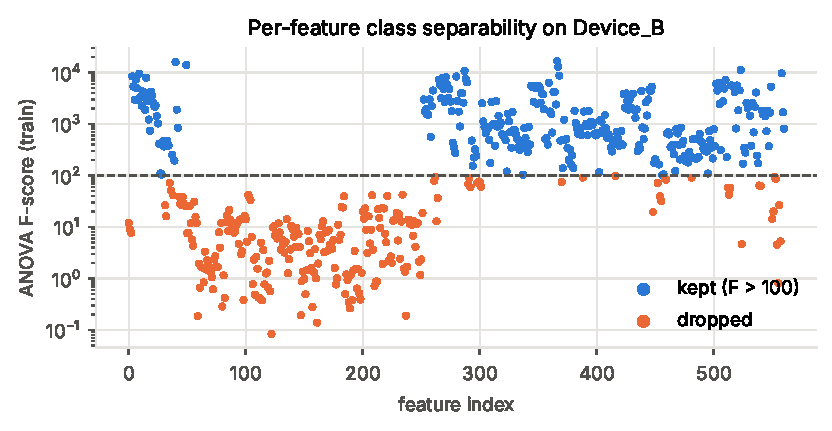
\includegraphics[width=\linewidth]{fscore.pdf}
  \caption{Per-feature ANOVA $F$ on Device\_B (log scale) and the selection threshold.}
  \label{fig:fscore}
\end{figure}

\begin{figure}[t]
  \centering
  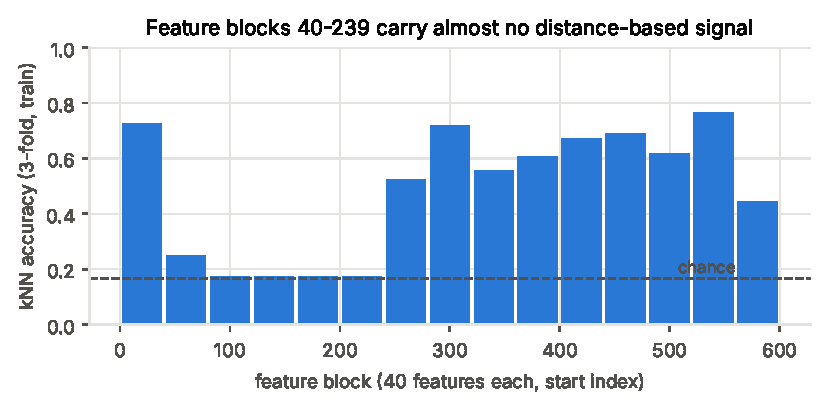
\includegraphics[width=\linewidth]{block_knn.pdf}
  \caption{kNN accuracy (3-fold, within Device\_B) using one 40-feature block at a time.}
  \label{fig:block_knn}
\end{figure}

\subsection{Pipeline}
\textbf{Per-device standardization.} A calibration offset $b_j$ and gain $a_j>0$ transform
feature $x_j$ into $a_jx_j+b_j$; its mean and standard deviation become $a_j\mu_j+b_j$ and
$a_j\sigma_j$, so
\begin{equation}
  \frac{(a_jx_j+b_j)-(a_j\mu_j+b_j)}{a_j\sigma_j}=\frac{x_j-\mu_j}{\sigma_j}.
\end{equation}
Standardizing every device with \emph{its own} statistics therefore cancels any per-feature
affine distortion; a scaler fitted on the training device cannot. Standardized values are
clipped to $\pm8$ (winsorizing~\cite{huber1981}) and missing values map to 0.

\textbf{Unsupervised device discovery.} Test files carry no device identity, and clustering on
all features would recover \emph{activities} (static vs.\ dynamic postures are well separated),
which per-cluster standardization would erase. We therefore cluster on \emph{probe features}:
the 25\,\% of features with the lowest training $F$-score, i.e.\ those least related to the
activity. Probes are robust-z-scored with training statistics, projected to two principal
components fitted on the test set, and clustered with $k$-means for $k=2\dots4$. A split is
accepted only if its silhouette~\cite{rousseeuw1987} is $\ge 0.8$ and every cluster holds
$\ge\max(30, 5\,\%\,N)$ records; otherwise the test set is one device. Clusters smaller than
30 fall back to the training statistics. On each validation half alone and on the training
data the rule correctly returns $k=1$ (small outlier groups are rejected by the size rule).
\Cref{fig:devices} shows the two discovered devices.

\begin{figure}[t]
  \centering
  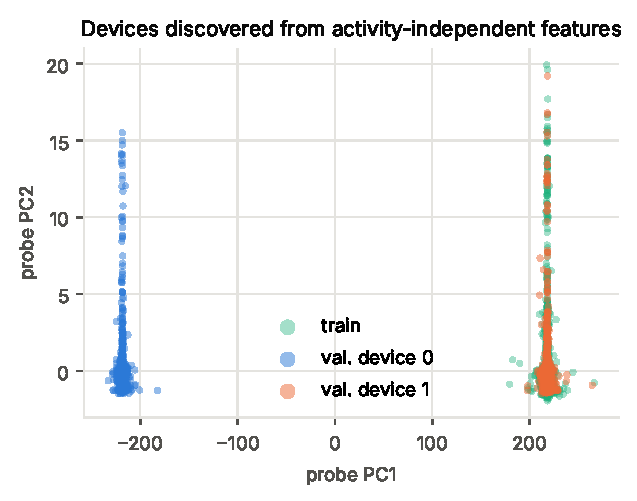
\includegraphics[width=0.85\linewidth]{device_clusters.pdf}
  \caption{Probe-feature PCA of the validation set: the discovered devices and the training data.}
  \label{fig:devices}
\end{figure}

\textbf{Feature selection.} On standardized, clipped training features we keep those with ANOVA
$F>\FThreshold$ (a univariate filter~\cite{guyon2003}), \NSelected{} of 561. The threshold is
not fragile: validation accuracy is flat for thresholds between 25 and 200 (\cref{fig:tuning}).

\textbf{Classifier.} An RBF SVM~\cite{cortes1995} with $C=\TunedC$ and $\gamma$=\texttt{scale}
(one-vs-one~\cite{hsu2002}, libsvm~\cite{chang2011libsvm}); \NSV{} support vectors; model file
\ModelMB\,MB.

\textbf{Inference and timing.} \texttt{infer.py} lists \texttt{1.csv}\dots\texttt{N.csv}
numerically, reads all files (untimed I/O, as the brief specifies), runs the one-off
adaptation (device discovery + statistics + one warm-up prediction, \FinalAdaptS\,s on
the validation set), then times each sample's standardization and prediction individually.
Each line of \texttt{time.txt} is that time plus the adaptation time divided by $N$, so no
computation is hidden. For speed the SVM decision is re-implemented in numpy: one
matrix--vector product gives all kernel values, a precomputed $15\times n_{SV}$ matrix gives
the 15 pairwise decisions, and a vote picks the class. It is verified identical to
scikit-learn~\cite{pedregosa2011} at training time and in the tests (byte-identical
\texttt{results.txt} on all validation files) and cuts per-sample latency by $\approx 3\times$.

\textbf{Engineering.} The code is one Python package with a module per stage (data,
preprocessing, features, models, evaluation, inference, experiments), strict type checking, 56
unit/integration tests on synthetic data, import-boundary contracts, continuous integration
that also builds the Docker image and runs it, and a Gradio demo for Hugging Face Spaces
(\HFLink). Source: \RepoLink.
